\documentclass[../main.tex]{subfiles}

\begin{document}
\begin{enumerate}[(a)]

\item ¿Cuál es la probabilidad de que la demanda mensual de Detergente2
en una sucursal en particular esté entre 12000 y 18000 unidades?

\begin{figure}[h]
\centering
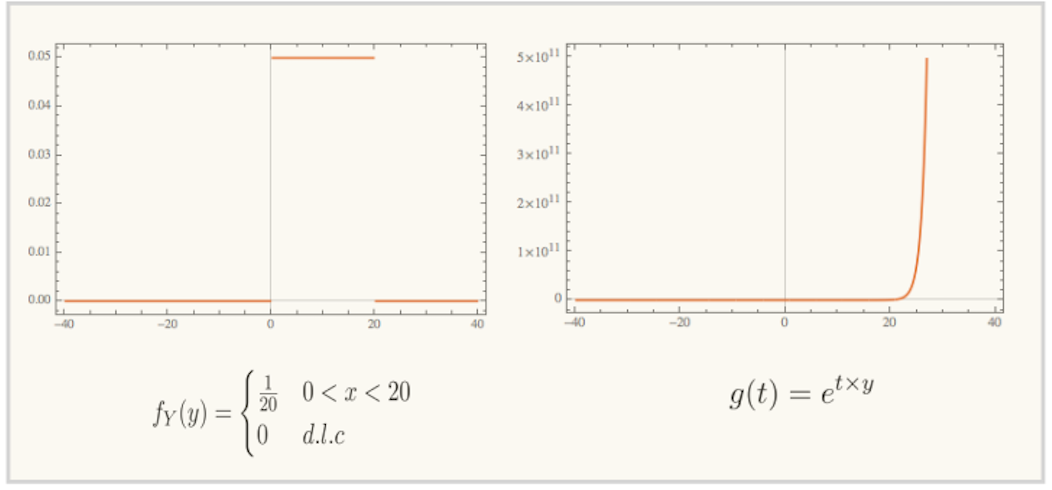
\includegraphics[width=8cm]{fig4-1}
\label{fig:img1}
\caption{Distribución triangular de X. $\mathbb{P}(12 < X < 18)$}
\end{figure}

$$\mathbb{P}(12 < X < 18) = 1 - [\mathbb{P}(X < 12) + \mathbb{P}(18 < X)]$$
$$\mathbb{P}(12 < X < 18) = 1 - \left[\frac{(6)(0.039)}{2} + \frac{(22)(0.0517)}{2}\right] = 0.3143$$

\item La empresa ha decidido examinar la demanda promedio mensual del
producto Detergente2, de 70 sucursales seleccionadas al azar. Calcule la
probabilidad de que la demanda mensual promedio en dichas sucursales sea
mayor a 21000 unidades.

Dado que $70 > 30$, es posible modelar el promedio como una distribución normal con parámetros: 
$$\mu = (6 + 15 + 40) / 3 = 20.33$$
$$\sigma = \sqrt{\frac{6^2+40^2+15^2+(6)(40)-(6)(15)-(40)(15)}{18}} = 7.19$$

Se quiere la probabilidad $\mathbb{P}(X > 21) = 1 - \mathbb{P}(X < 21)$. \\
$$Z = \frac{21-20.33}{(7.18 / \sqrt{70})} = 0.78$$

$$\mathbb{P}(X > 21) = 1 - \mathbb{P}(X < 21) = 1 - \mathbb{P}(Z < 0.78) = 0.7823$$

\pagebreak

\item Si se eligen 35 sucursales al azar, calcule la probabilidad de que la
demanda mensual total del Detergente2 en estas sea menor a 650000 unidades.\\

Dado que 35 > 30, por el teorema del limite central, se sabe que $X_{n}$, se puede modelar como una distribución normal con parámetros equivalentes a multiplicar por $n = 35$, la media y la varianza de la distribución triangular, es decir:

$$\mu = n \times \mu_{Tri} = (35) \times (20.33) = 711.55$$
$$\sigma = n \times \sigma_{Tri} = (35) \times (7.19) = 251.65$$

$$\mathbb{P}(X_{n} < 650000) = \mathbb{P}\left(Z < \frac{650-711.55}{251.65}\right) = 1 - \mathbb{P}(Z < 0.24) = 0.4052$$

\item Si se sabe que el precio unitario del producto Detergente2 es de \$1200
pesos y que el costo logístico mensual, asociado únicamente a este producto, en
cada una de las sucursales se comporta como una variable aleatoria normal $\mathcal{N} (\mu = 20.5 , \sigma = 5.6)$ en millones de pesos, ¿se esperaría que las ventas promedio
mensuales del producto en todas las sucursales del país sean suficientes para
solventar dicho costo para la empresa?\\

Las ventas promedio en todas las sucursales están dadas por el valor esperado de la variable $X$; demanda mensual con distribución triangular con $\mu = 20.33$ miles de unidades. Ventas promedio $= (1200)(20330) = 24396000$. Como las ventas promedio son mayores al costo promedio ($24396000 > 20500000$), si se espera que las ventas fueran suficientes para solventar el costo.

\end{enumerate}
\end{document}
